\documentclass{draft-sbml-paper}
\usepackage{authblk} % managing affiliations
\usepackage{wrapfig}

% This create the box section. We should probably be more clever and use the titlesec package from l3-packages-table. Everything will be reformatted before submission anyway
\newcounter{mybox}
\newcommand{\mybox}[1]{%
   \refstepcounter{mybox}%
   \noindent\textbf{\Large \rule{1cm}{0.4pt}~Box~\themybox{}. #1~\hrulefill}%
}%

\makeatletter
  \renewcommand\Affilfont{\small}
  % \renewcommand\maketitle{\AB@maketitle} % revert \maketitle to its old definition
  \renewcommand\AB@affilsepx{\quad\protect\Affilfont} % put affiliations into one line
  
  \hypersetup{
    pdfpagemode={UseNone},
    pdfcenterwindow={true},
    pdfview={FitV},
    pdffitwindow={true},
    pdfwindowui={false},
    pdfstartview={FitV},
    pdfnewwindow={false},
    pdfdisplaydoctitle={true},
    pdfhighlight={/P},
    pdflang={en},
    unicode={true},
  }
  \AtBeginDocument{\hypersetup{pdftitle=\@title, pdfsubject={Molecular Systems Biology}}}
\makeatother

\title{SBML Level 3: an extensible format for the exchange and reuse\\of biological models}

\author[1]{\emph{List of authors here}}

% ======================================================================

\begin{document}

\maketitle

\begin{abstract}
Systems biology has experienced dramatic growth in the number, size and complexity of computational models describing biology. To reproduce simulation results and reuse models, researchers need to exchange precise and unambiguous descriptions of model structure and meaning. SBML (the Systems Biology Markup Language) is a community-developed format for this purpose. The latest edition, called SBML Level~3, has a modular structure, with a core suited to representing reaction-based models, and packages that extend the core with features suited for a variety of model types. Examples include constraint-based models, reaction-diffusion models, logical network models, and rule-based models. SBML and its rich software ecosystem have transformed the way systems biologists build and interact with models, and has played an important role in increasing model interoperability and reuse over the past two decades. More recently, a rise of multiscale models of whole cells and organs, and new data sources such as single cells measurements and live imaging, have precipitated new ways of integrating data and models. SBML Level~3 provides the foundation needed to support this evolution.

\vspace*{0.25in}\noindent
\begin{tabular}{@{}ll@{}}
  \textbf{MSB subject category}: & Methods \& Resources \\
  \textbf{Keywords}: & methods / software / biological modeling \\
  \textbf{Running title}:        & SBML Level 3\\
  \textbf{Abstract word count}:  & 172 \\
  \textbf{Body word count (using \texttt{texcount})}: & 5420\\
\end{tabular}

\end{abstract}

\clearpage

% ======================================================================
\section*{Introduction}
% ======================================================================

Systems modeling and numerical simulations in biology can be traced to the mid-20\textsuperscript{th} century. Though general theorizing about systems began earlier, the application of systems analysis to biology gained attention in the 1950's thanks to the work of biologists such as Bertalanffy and Kacser~\citep{Von_Bertalanffy1950-dy, Von_Bertalanffy1950-wa, Kacser1957-ox}. The era of numerical simulations in biology truly began with the landmark works of Chance on enzyme kinetics~\citep{chance1952mechanism, chance1940kinetics}, Hodgkin and Huxley on the molecular basis of neuronal transmission~\citep{hodgkin1952quantitative}, and Turing on the chemical basis of morphogenesis~\citep{turing1990chemical}. Since then, the number and variety of models have grown in all of the life sciences. As precise descriptions of phenomena that can be simulated, analyzed, and compared to experimental data, models provide unique insights that can confirm or refute hypotheses, suggest new experiments, and identify refinements to the models~\citep{Heinrich1996, le_novere_2015}.

The availability of more data about biological mechanisms, more powerful modeling methods, and dramatically increased computing power, led to the rise of systems biology as a compelling research theme around the turn of the millennium~\citep{kitano2000perspectives, ideker2001new}. Though computational models were at first published as printed equations in journal articles, the desire to reuse an ever-increasing number of models called for digital formats that could be communicated directly between different software systems and databases, and easily exchanged between scientists~\citep[topics of interest as early as the 1960's; c.f.][]{Garfinkel1969construction}. This drove efforts to create tool-\emph{independent} ways of representing models that could avoid the potential for human translation errors and provide a common starting point for simulations and analyses regardless of the software used~\citep{Lloyd2004-fd, Goddard2001-ix, hucka_2001}. One such effort was SBML, the Systems Biology Markup Language. Its initial design was motivated by discussions to create a ``metabolic model file format'' following a 1999 workshop~\citep{Cornish-Bowden2000technological}. A distributed community thereafter discussed ideas that informed work at Caltech in late 1999/early 2000 and led (after a series of public drafts) to the specification of the official version of SBML Level 1 Version 1 being released in March 2001~\citep{hucka_2003}.

While SBML was initially developed to exchange non-spatial compartmental models of biochemical reaction networks primarily formulated in terms of chemical kinetics~\citep{hucka_2002}, it was always understood that there existed more types of models than the initial version of SBML could represent directly. However, seeking community consensus on a limited set of simpler features, which could be readily implemented in software at the time, was deemed a more pragmatic strategy. A deliberate decision was taken to delay the addition of more advanced capabilities to later in time.  As a result, SBML has evolved in stages in a community-driven fashion that has benefited from the efforts of many researchers worldwide over nearly two decades.  Over time, the community saw the need to support a broader range of model types, modeling paradigms, and research areas. In addition to reaction-diffusion models, alternative modeling frameworks have risen in popularity in the past decade~\citep{Machado2011modelinga}. These needs drove a profound change in SBML's structure: a facility to permit layering the core of SBML with new features suited to more types of models, together with a way for individual models to identify which sets of extensions they need for proper interpretation. The release of SBML Level~3 in 2010~\citep{Hucka2015} has provided a new foundation to enable the exchange of a greater variety of models in various domains of biology (\autoref{level-3-diagram}).

In this article, we describe SBML Level~3's structure, its support for different model features, its community-oriented development process, its impact, and finally, forthcoming challenges.

\begin{figure}[b]
  \center
  \includegraphics[width=\textwidth]{res/SBML-Level3-v08.png}
\caption{SBML Level 3 consists of a core (center) and specialized SBML Level~3 \emph{packages} (in blue), which provide syntactical constructs to support additional modeling approaches. The packages support new types of modeling (in gray) needed for large and complex models such as those used in various domains and fields of biology (in red). The meanings of SBML package labels such as ``fbc'' are given in \autoref{packages}, with additional package information in Box~1.}
\label{level-3-diagram}
\end{figure}

\clearpage
\newpage

% ======================================================================
\section*{The structure of SBML}
\label{sec:sbml}
% ======================================================================

The core of SBML is focused on encoding models in which entities are located in containers and are acted upon by processes that produce modified or new entities.  The containers do not need to correspond to physical structures; they can be conceptual or abstract.  Additional constructs allow parameters, initial conditions, other variables, and other mathematical relationships to be defined.  In the most common type of model, the ``entities'' are biochemical substances, the ``containers'' are well-mixed and spatially homogenous, and the ``processes'' are biochemical reactions happening within or between the containers.  This originally led to the SBML constructs being named \emph{species}, \emph{compartments}, and \emph{reactions}, respectively (Figure \ref{fig:examples-sbml}B), but these names are a historical artifact and belie the generality of the underlying scheme.  Software applications can map the names to other concepts to better suit their purposes.  For instance, the ``species'' could be mapped to populations of molecules, cells, or even organisms.

Modelers and software applications are encouraged to use SBML's reaction construct to define a model's behavior, in preference to formulating the model explicitly as a system of equations.  This gives users freedom to convert the representation into an end format they prefer---a simpler operation than going from equations to another form such as a reaction network, which requires inferring reaction systems~\citep{Fages2015inferring}.  The approach also naturally handles models where reaction kinetics are unknown or unneeded, such as interaction maps~\citep[e.g.,][]{thiele2013community}, and supports the elaboration of the reaction construct using SBML packages (see below).  That said, the use of reactions is optional, and SBML provides features sufficient for encoding a large diversity of purely mathematical models too.  Whether using reactions or not, values of model variables and their changes over time may be fixed or determined by mathematical expressions, either before or during simulation, continuously or in response to discrete events, with or without time delays.  Units of measurement can be specified for all entities and values; in addition to adding a layer of essential physical knowledge (after all, how else could one interpret whether a time course is in milliseconds or years?), information about units can be used to validate the relationships expressed in a model.  Units also facilitate reuse of models and components, interconnection of models, conversion of models between different frameworks, and integration of data with models.

SBML does not dictate which framework must be used to analyze or simulate a model; in fact, it lacks any explicit way to specify what is done with a model---whether to run simulations or other types of analyses, how to run them, or how to present the results---because externalizing this information enhances model reusability and permits independent innovation in separate but complementary formats.  Two of the most popular methods for time-course simulation are both commonly used: one is numerical integration of differential equations created from the reactions and other relationships affecting model variables, and the other is simulating the time evolution of the model as a stochastic system via algorithms such as the one developed by~\cite{gillespie1977exact}.  Alternative approaches are also in use, particularly when a model is enhanced with SBML packages.  The separation of models and protocols also facilitates the development of virtual experiments that can be applied to multiple models~\citep{Cooper2015call}.

Any element of an SBML model can be elaborated using optional machine-readable metadata as well as human-readable notes.  For metadata, two schemes are supported.  The first is direct labeling with terms from the Systems Biology Ontology~\citep[SBO;][]{courtot2011controlled}, which allows the mathematical semantics of every element of a model to be precisely specified.  The second scheme uses semantic web technologies and provides greater flexibility to capture more information.  For instance, a molecular species in a model can be linked to a UniProt entry~\citep{uniprot2017} if it represents a protein, or to ChEBI entry~\citep{hastings2013chebi} if it represents a simple chemical.  Gene Ontology terms~\citep[GO;][]{ashburner2000gene} can be attached to species, compartments, and mathematical elements representing biological processes and functions.  Clerical data such as identities of creators can be added to facilitate tracking and versioning.  To help standardize how annotations are stored, SBML encourages the use of guidelines and resources established for this purpose~\citep{le_novere_2005, Laibe2007miriam, Juty2012identifiers}.  Finally, software tools can also use annotations to encode tool-specific data in their own formats, thus providing a way to capture data that might otherwise be lost if it has no other place to be stored.  Annotations thereby help enrich the meaning of model components, facilitate the understanding and reuse of models, and help software work with SBML more flexibly~\citep{krause2011chapter, schulz2011retrieval, Lister2010annotation, Schulz2012propagating, Swainston2009libannotationsbml}.

\clearpage

\begin{figure}[htb]
  \center
  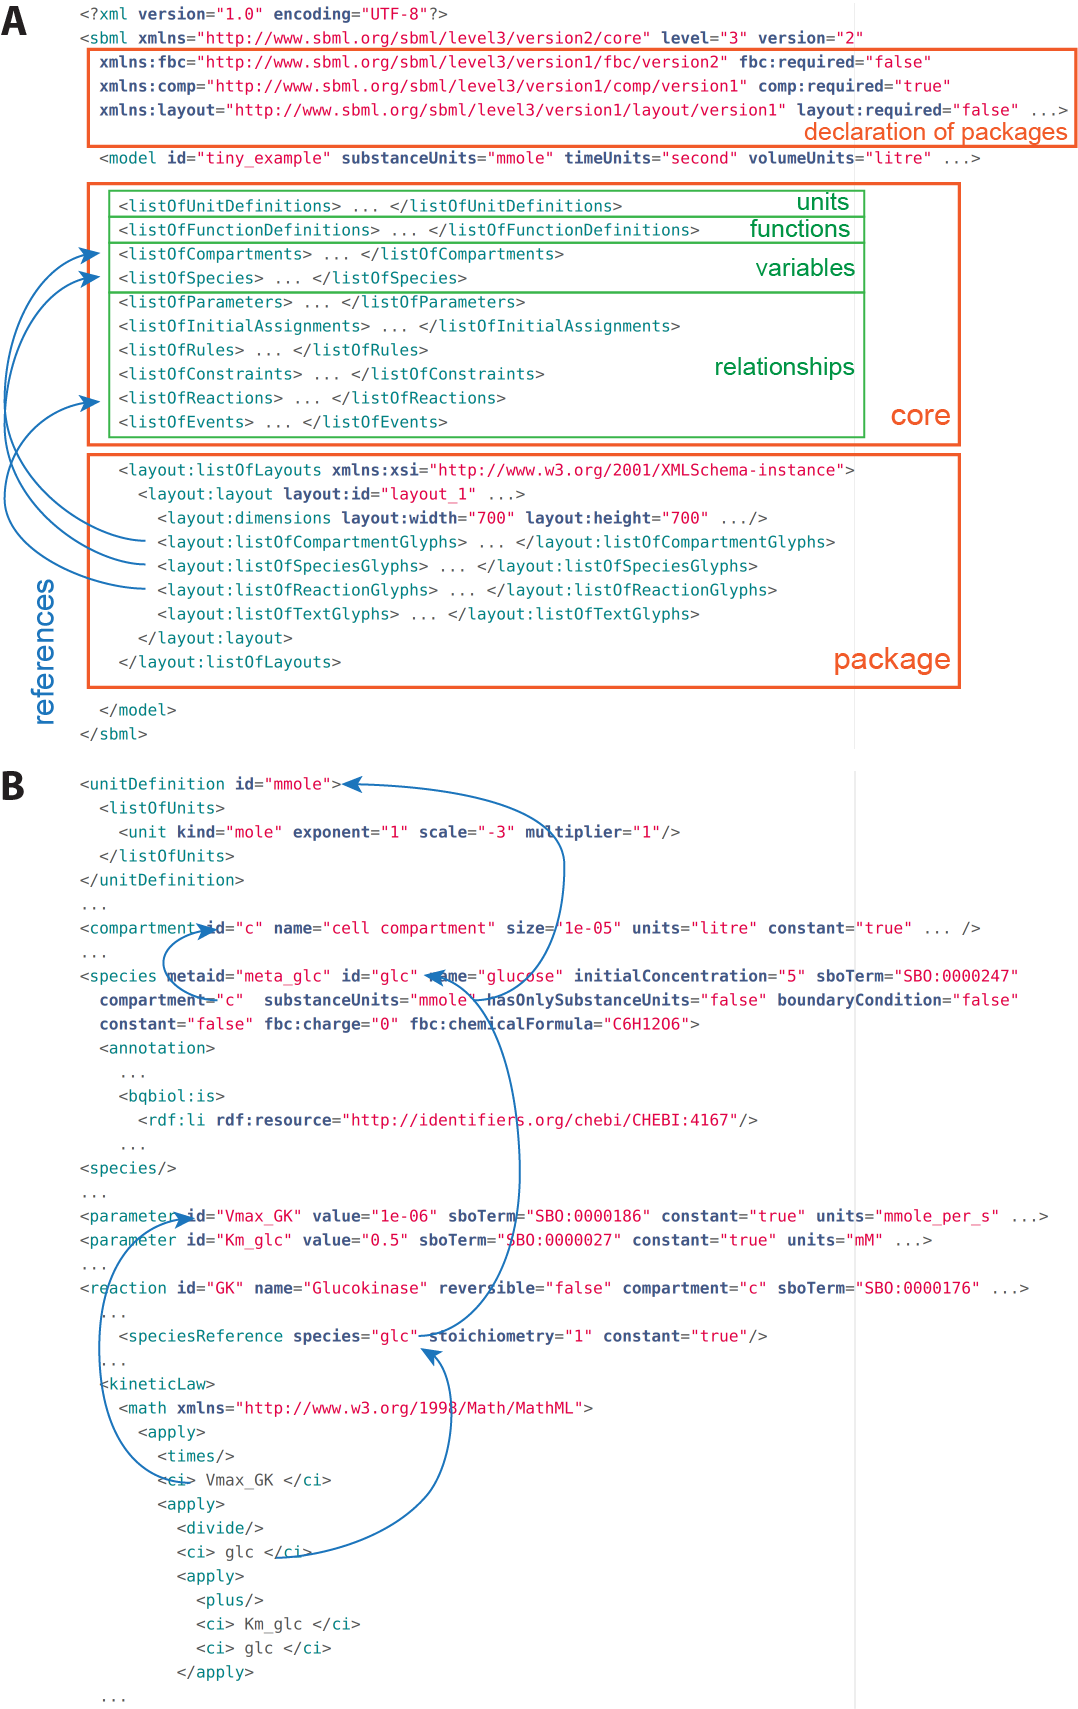
\includegraphics[width=.79\textwidth]{res/SBML_XML_example_v03.png}
  \caption{A closer look at SBML. A) Fragments of the global structure of an SBML file. In this example, the use of several SBML packages is declared in the file header. Model elements in the file include the descriptions of model variables, as well as their relationships.  Elements of the same type are collected into ``ListOf'' elements; \eg model parameters are in the ListOfParameters element. SBML package elements can refer to elements in the SBML Core as necessary. B) Model elements are linked through unique identifiers used in the mathematical constructs and the elements describing the reactions, the molecular species, and their localization. The full model for this example is available in BioModels Database~\citep{chelliah2014biomodels} as the model with identifier \texttt{MODEL1904090001}.}
\label{fig:examples-sbml}
\end{figure}


\clearpage
\newpage

% ======================================================================
\section*{SBML Level 3's modularity and breadth}\label{sec:modularity}
% ======================================================================

Constant evolution in scientific methods presents challenges for the creation of software tools.  One challenge arises because the creation of new standards requires labor, testing and time.  This often leads standardization efforts to lag behind the latest technical developments in a constantly-moving field.  A second challenge is that users want support for new methods and standards in software tools, which pressures developers to implement support quickly.  Combined with the first challenge, sometimes this means that problems with a standard's definition are not discovered until more developers attempt to use it in different situations, which in turn often means that revisions to a standard are needed after it is published.  Finally, another challenge is that software development often takes place under resource constraints (\eg funding and time), limiting the scope of work that software developers can undertake---including, sometimes, limiting on how many features of a standard they can support in their software.

The SBML community sought to address these challenges by putting in place certain structural features in SBML's development process.  The first is the notion of \emph{Levels}.  A Level in SBML is an attempt to provide a given set of features for describing models, with higher Levels providing more powerful features.  For example, the ability to express discrete events was added to SBML Level~2 but does not exist in Level~1.  SBML Levels are mostly upwardly compatible, in the sense that the vast majority of models encoded in Level $n$ can be translated to Level $n+1$.  \emph{Versions} are used to introduce refinements to a given Level to account for realizations that come from real-life use of SBML.  Finally, SBML Level~3 introduced an extensible modular architecture consisting of a central set of fixed features (named \emph{SBML Level~3 Core}), and a scheme for adding \emph{packages} that can augment the \emph{Core} by extending existing elements, adding new elements, and adjusting the meaning or scope of elements.  A model declares which packages it uses in order to guide its interpretation by software applications.  If a software tool detects the presence of packages that it does not support, it may inform users if it cannot work with the model.  Together, these three features (Levels, Versions, packages) help address the challenges discussed above: they ease coping with evolution in methods by collecting significant changes into discrete stages (SBML Levels), they help deal with the inevitable need for revisions (Versions within Levels), and they allow developers to limit the feature set they implement (SBML Levels on the one hand, and SBML Level~3 packages on the other hand).

Packages allow SBML Level~3 to represent many model types and characteristics in a more natural way than if they had to be shoehorned into SBML Core constructs exclusively.  Twelve packages have been proposed to date (\autoref{packages}); six have been fully developed into consensus specifications and are used by at least two software implementations (Box~\ref{box:packages}), and another three have draft specifications in use by software tools.  New packages can be developed independently, within dedicated communities, at a pace that suits them.  This was the case for logical modeling with the CoLoMoTo community~\citep{naldi2015cooperative}, constraint-based modeling within the COBRA community~\citep{Ebrahim2015}, and rule-based modeling with a community of like-minded software creators~\citep{Blinov2004, Palmisano2014multistate, zhang2013simmune}.  The approach of letting models declare the SBML packages needed for their full interpretation is useful because even if a software application does not implement support for a given package, the application may still be able to interpret \emph{some} fundamental aspects of the model by understanding Level~3 Core (and perhaps other packages used by the model).  For example, given a model that uses SBML ``spatial'', the reaction network of a reaction-diffusion model may still provide useful information even without the spatial context.

Though this modular approach has benefits, it is not without potential pitfalls.  The main risks are fragmentation of the community, and incompatibility of packages due to complex feature dependencies.  The SBML community addressed the former by maintaining communications between package developers.  As for the latter, API libraries (see Box~\ref{box:software}) can handle \emph{some} combinations of packages and hide some of the complexity.  Still, there remain some combinations of packages that are not fully understood, and it remains for future work to define how (if ever) they can be combined use in a single model.

\clearpage
\newpage
% Master File: main.tex -*- TeX-master: "main" -*-

\definecolor{ourgray}{rgb}{0.3,0.3,0.3}

\newcommand{\symbolcolor}{black}

\newcommand{\notstarted}    {\textcolor{\symbolcolor}{\scalebox{1.25}{\danger}\xspace}}
\newcommand{\suspended}     {\textcolor{\symbolcolor}{\hspace{3.5pt}\scalebox{1.25}{\danger}*}}
\newcommand{\inprogress}    {\textcolor{\symbolcolor}{\raisebox{-2.5pt}{\scalebox{1.6}{\clock}}\xspace}}
\newcommand{\done}          {\textcolor{\symbolcolor}{\scalebox{1.3}{\checkmark}\xspace}}
\newcommand{\notapplicable} {\textcolor{\symbolcolor}{n/a\xspace}}

\newcommand{\released}      {\textcolor{\symbolcolor}{\CIRCLE\xspace}}
\newcommand{\notreleased}   {\textcolor{\symbolcolor}{\Circle\xspace}}

\begin{sidewaystable}
  \centering
  \rowcolors{3}{}{rowgray}
  \renewcommand{\tabcolsep}{4pt}
  \renewcommand{\arraystretch}{1.3}
  \caption{Overview of SBML Level~3 packages and their release and development statuses.  Symbols: \protect\released = released; \protect\notreleased = not released; \protect\done = complete; \protect\inprogress = in progress; \newline\protect\notapplicable = not applicable. Spec.\ = specification.}
  \begin{tabular}{m{0.12in}>{\raggedright}m{2in}>{\raggedright}m{0.47in}>{\raggedright}m{4.3in}>{\hspace*{3pt}}>{\hspace*{-5pt}}c>{\hspace*{-4pt}}c>{\hspace*{-4pt}}c>{\hspace*{-3pt}}>{\hspace*{1pt}}c}
    \toprule
    &                       &                   &                  & \textbf{Spec.} & \textbf{libSBML} & \textbf{JSBML}   & \textbf{Test} \\[-4pt]
    & \textbf{Package name} & \textbf{Label} & \textbf{Purpose} & \textbf{Status}        & \textbf{Support} & \textbf{Support} & \textbf{Suite} \\
    \midrule
\released
& Flux Balance Constraints
    & fbc
    & Define constraint-based models (also known as steady-state models).
    & \done
    & \done
    & \done
    & \done
    \\    
\released
& Groups
    & groups
    & Collect elements together for annotation purposes.  Groups have no mathematical meaning and do not affect simulations.
    & \done
    & \done
    & \done
    & \notapplicable
    \\
\released
& Hierarchical Model Composition
    & comp
    & Define models composed of other models. Those ``submodels'' can be stored in the same file or as separate files.
    & \done
    & \done
    & \done
    & \done
    \\
\released
& Layout
    & layout
    & Store positions and sizes of model components in drawings of network diagrams of SBML models. (Cf.\ Rendering package.)
    & \done
    & \done
    & \done
    & \notapplicable
    \\
\released
& Multistate, Multicomponent, and Multicompartment Species
    & multi
    & Define complex features such as states or binding sites on molecular species, optionally in combination with rule-based processes.
    & \done
    & \done
    & \done
    & \inprogress
    \\
\released
& Qualitative Models
    & qual
    & Define logical networks, Petri Nets, and similar models in which the numerical values of SBML species represent qualitative activity levels rather than amounts or concentrations of molecules.
    & \done
    & \done
    & \done
    & \inprogress
    \\
\released
& Rendering
    & render
    & Extend the Layout package to enable storing graphical symbols and styles, curves, colors, and gradients in network diagrams.
    & \done
    & \done
    & \done
    & \notapplicable
    \\
\hline
\notreleased
& Arrays
    & arrays
    & Define arrays of elements, such as arrays of compartments. (Core SBML Level~3 supports only scalar values.)
    & \inprogress
    & \done
    & \done
    & \inprogress
    \\
\notreleased
& Distributions
    & distrib
    & Define statistical distributions for quantitative values. (Core SBML does not enable indicating value ranges or distributions.)
    & \inprogress
    & \done
    & \done
    & \inprogress
    \\
\notreleased
& Dynamical Processes
    & dyn
    & Describe the creation, destruction, and movement of model elements during simulation.
    & \inprogress
    & \done
    & \done
    & \inprogress
    \\
\notreleased
& Extended math
    & math
    & Add additional syntactic constructs not included in the subset of MathML used by SBML Level~3 Core for mathematical expressions.
    & \inprogress
    & \inprogress
    & \inprogress
    & \inprogress
    \\    
\notreleased
& Spatial Processes
    & spatial
    & Define spatially-inhomogeneous compartment geometries and processes such as diffusion.
    & \inprogress 
    & \done
    & \done
    & \inprogress
    \\
    \bottomrule
  \end{tabular}
  \label{packages}
\end{sidewaystable}


\clearpage
\newpage
% **********************************************************************
\mybox{SBML Level~3 packages officially part of the standard}\label{box:packages}
% **********************************************************************

\textbf{Hierarchical Model Composition}~~~~The ``comp'' package~\citep{Smith2015} allows users to build models from other complete models or from model fragments as a way to manage complexity and construct composite models. ``Submodels'' can be described within the same SBML file or linked from external files. A submodel can act as a template, and the same definition can be reused multiple times in other models to avoid duplication and enable reuse of parts. The ``comp'' package also enables submodels to have explicit interfaces (known as \emph{ports}) for optional black-box encapsulation. Finally, ``comp'' was designed so that a hierarchical model can be converted into a single SBML model that does not use any ``comp'' features,  making it readable by software that does not directly support the package. The library libSBML~\citep{bornstein2008libsbml} provides a facility to do this.

\textbf{Flux Balance Constraints}~~~~The ``fbc'' package~\citep{Olivier2018a} provides a means of encoding constraint-based models and optimizations, such as is done in Flux Balance Analysis ~\citep{Bordbar2014a}. Constructs in the ``fbc'' package allow for the definition of a list of objectives for minimization or maximization, as well as flux bounds on reactions and gene-reaction mappings. Additional information such as chemical formula and charge enable further model analyses, including calculation of reaction mass balances, electron leaks, or implausible sources of matter.

\textbf{Groups}~~~~The ``groups'' package~\citep{hucka2016sbml} provides constructs to describe conceptual relationships between model elements. Groupings can indicate classification, partonomy, or merely a collection of things; a group's meaning can be specified using semantic annotations.  Groups have no semantic meaning and cannot influence the mathematical interpretation of an SBML model.

\textbf{Multistate, Multicomponent and Multicompartment Species}~~~~The ``multi'' package~\citep{zhang2018multi} manages the combinatorics produced by entities either composed of multiple components, such as molecular complexes, or that can exist in multiple states, such as proteins with post-translational modifications. With the ``multi'' package, rules can be defined for how reactions depend on the states of the entities and their locations. The package adds syntactic constructs for molecular species types, compartment types, features, binding sites, and bonds.  Entire families of molecular complexes sharing certain properties can be defined using patterns created using these constructs.

\textbf{Qualitative Models}~~~~The ``qual'' package~\citep{Chaouiya2015sbml} provides constructs to encode models whose dynamics can be represented by discrete reachable states connected by state transitions denoting qualitative updates of model elements. Examples include logical regulatory networks (Boolean or multi-valued~\citep{abou2016logical}) and Petri nets~\citep{chaouiya2007petri}. The ``qual'' package introduces SBML elements to allow the definition of qualitative species, which are used to associate discrete levels of activities with entity pools, as well as transitions, which define the possible changes between states in the transition graph.

\textbf{Layout \& Rendering}~~~~The ``layout''~\citep{Gauges2015} and ``render''~\citep{Bergmann2018sbml} packages extend SBML to allow graphical representations of networks or pathways to be stored within SBML files. The ``layout'' package enables the encoding of positions and sizes of graphical elements such as nodes and lines, while the information about colors, fonts, etc., are defined by the ``render'' package. This separation presents several advantages. For example, applications can offer multiple styles for visualizing the same layout of a network map. Most of the essential aspects of a network diagram can be expressed using just the ``layout'' package, and thus tools do not necessarily have to implement a full graphics environment if they do not need to support customizing a diagram's look-and-feel.

\hrulefill

\newpage
% ======================================================================
\section*{SBML as a community standard}
% ======================================================================

SBML's success can be attributed largely to its community-based development and its consensus-oriented approach. SBML has always been developed through engagement with its user community to achieve goals expressed by that same community. To resolve occasionally conflicting technical demands, a guiding principle has been to seek consensus between different viewpoints and the needs of different groups, to find a middle ground that would be---while perhaps not a perfect solution---an \emph{acceptable} and \emph{usable} solution. This attracted the researchers and software developers who constitute SBML's foremost stakeholders. By using SBML in everything from software to textbooks~\citep[e.g.,][]{Cesario2011cancer, Sullivan2012introduction, Wilkinson2018stochastic, Klipp2016systems, Liu2009systems, Choi2008introduction, Sauro2014systems}, they helped drive further development to face the real needs expressed by the people who have those needs.  This engagement allowed faster feedback from users to developers, and helped produce a rich toolkit of software and other resources that facilitate SBML's incorporation into software (Box~\ref{box:software}).

Over the years, the community has designed rules to organize its governance, develop and maintain the specifications, and facilitate collaboration among users.  The development of SBML and its Level~3 packages is shepherded by the SBML Editors, a group of community-elected volunteers serving terms of three years, who follow a written and public process detailed on the web portal SBML.org\footnote{\url{http://sbml.org/Documents/SBML_Development_Process}}.  SBML editors write or review SBML specification documents, organize discussions and vote on specific technical issues, and enact the decisions of the community.  Major proposed changes to the specifications and packages are discussed by the community via the SBML mailing lists\footnote{\url{http://sbml.org/Forums/}} as well as during annual face-to-face meetings.  The community currently comes together twice a year within the context of meetings organized by COMBINE~\citep[the Computational Modeling in Biology Network;][]{Hucka2015promotinga}.  \emph{HARMONY} (the Hackathon on Resources for Modeling in Biology) is a codefest that focuses on the development of software, in particular via the development of libraries, tools and specifications; by contrast, the \emph{COMBINE Forum} meetings focus on the presentation of novel relevant tools and the discussion of proposed features.  In addition to these general meetings, special SBML working groups are organized as needed to drive SBML package development.

One of COMBINE's core activities is to maintain a list of persistent URLs for all specification documents developed by standardization groups under the COMBINE umbrella\footnote{\url{http://co.mbine.org/standards/specifications/}}, including the SBML specifications, so that users can refer unambiguously to the precise version and release of a given specification document.  FAIRsharing, a broader community network that covers life sciences more comprehensively~\citep{Sansone2019fairsharing}, maintains interconnected and organized collections of resources in many areas, including curated links between SBML and many associated funders, databases, and standards\footnote{\url{https://fairsharing.org/FAIRsharing.9qv71f}}.

\clearpage
\newpage

% **********************************************************************
\mybox{Software infrastructure for SBML}\label{box:software}
% **********************************************************************

\newcommand{\tighturl}[1]{\textls[-20]{\url{#1}}}

\begin{tabular} {@{}c|c@{}}
    \textbf{Application Programming Interface (API)} & \textbf{Test Suite} \\
\begin{tabular} {P{3.1 in}}
Programming libraries help to read, write, manipulate, validate, and transform SBML
\begin{enumerate}
	\item LibSBML~\citep{bornstein2008libsbml} 
(\tighturl{http://sbml.org/Software/libSBML}) is written in C++ and offers language interfaces for C, C++, C\#, Java, JavaScript, MATLAB, Octave, Perl, PHP, Python, R and Ruby.

	\item  JSBML~\citep{Rodriguez2015} (\tighturl{http://sbml.org/Software/JSBML}) is a pure-Java based implementation.
\end{enumerate}
Both libraries:
\begin{itemize}
	\item Support all levels and versions of SBML
	\item Support all SBML Level~3 packages
	\item Use LGPL License
\end{itemize}
\end{tabular}
&
\begin{tabular} {P{2.9 in}}
An SBML Test Suite (\tighturl{http://sbml.org/Software/SBML_Test_Suite}) 
helps developers support SBML correctly and helps users check software compliance
\begin{enumerate}
\item Thousands of test cases for
\begin{itemize}
	\item Semantic interpretation of models (using results from both deterministic and stochastic simulation)
	\item Syntactic correctness
\end{itemize}
	\item A graphical front end that enables test cases to be filtered by Level/Version and a range of test tags. 
	\item An online database where test results can be uploaded and compared with results from other simulators.
\end{enumerate}
\end{tabular}
\\
\hline
    \vspace*{0.5ex}\textbf{Validation Facilities} & \textbf{Conversion Facilities} \\
\begin{tabular} {P{3.1 in}}
Validation software can check files for compliance to the definition of SBML
\begin{enumerate}
	\item API libraries include built-in validation
	\item Online validator has simple user interface (\mbox{\tighturl{http://sbml.org/Facilities/Validator}})
	\item Web services support software access
\end{enumerate}

Validation ensures compliance with
\begin{itemize}
	\item SBML syntax
	\item SBML validation rules published as part of each accepted SBML specification
\end{itemize}
\end{tabular}
&
\begin{tabular} {P{2.9 in}}
Converters (\tighturl{http://sbml.org/Software/Converters}) can translate certain other formats to SBML or vice versa
\begin{enumerate}
      \item Standalone conversion tools support format conversions from formats that include MATLAB~\citep[using MOCCASIN,][]{gomez2016moccasin}, BioPAX~\citep[using BioPAX2SBML,][]{Buchel2012qualitative}, and others
      \item Online services such as SBFC~\citep{Rodriguez2016systems} convert uploaded files to a variety of formats
      \item API libraries such as libSBML provide built-in converters between different SBML Levels/Versions and different SBML constructs
\end{enumerate}
\end{tabular}
\\
\hline
\multicolumn{2}{c} {
\textbf{Software Guide} 
}
\\
\multicolumn{2}{c}{
\begin{tabular} {P{6in}}
A catalog (\tighturl{http://sbml.org/SBML_Software_Guide}) of software applications, libraries and online services known to support SBML---over 290 entries to date
\begin{enumerate}
	\item A tabular interface highlights supported SBML features of each software system
	\item A list interface displays human-readable summaries of software systems
% 	\item Online gallery of screenshots (where provided)
\end{enumerate}
\end{tabular}
}
\end{tabular}


% 2019-04-22 <mhucka@caltech.edu>
% We need to shorten the paper, and this box doesn't seem essential.

% **********************************************************************
% \mybox{Package development process}\label{box:process}
% **********************************************************************

% \begin{wrapfigure}[34]{r}{0.5\textwidth}
%   \begin{center}
%     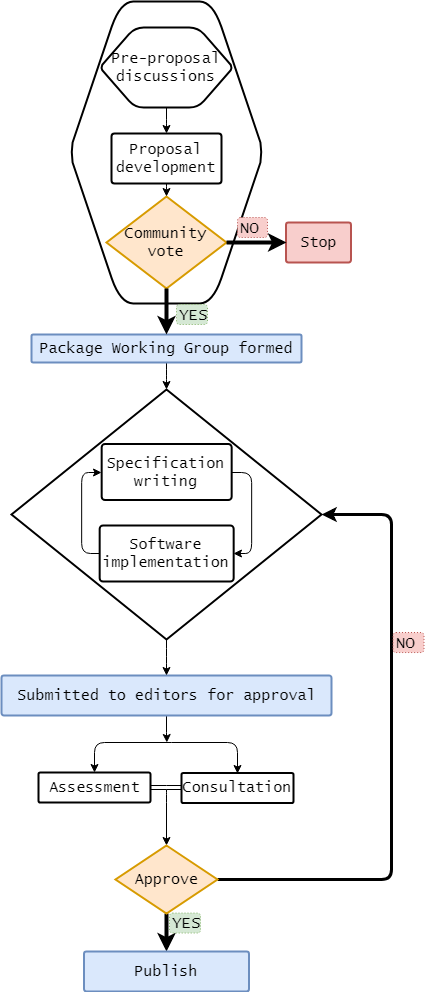
\includegraphics{res/Pkg_develop_v2.png}
%   \end{center}
% \end{wrapfigure}

% \textbf{Package proposal stage}\newline
% The SBML Editors follow a written \emph{SBML Development Process}, which includes a set of procedures that allows anyone to propose a new SBML package.  Proposals may be as detailed as the authors wish, but must include a description of the need to be served by the package and a general explanation of how the package will address that need.  Proposals are first voted on by the SBML community using a set of criteria that indicate that the area the package intends to address is appropriate, and that the proposed approach seems viable.

% \textbf{Package development stage}\newline
% Once a proposal has been approved, a \emph{package working group} (PWG) is formed and a dedicated mailing list established. All interested parties are encouraged to subscribe. Members of the PWG work on both specification and implementation, iterating on both following decisions made at each point. Once members have finalized the specification, they submit it to the SBML Editors, including a cover letter detailing the implementations.

% \textbf{Editor approval stage}\newline
% The SBML Editors review the specification for clarity and completeness. They document the exchange of models between implementations and, where appropriate, check that the results of simulation/analysis are reproducible. They finally accept the package as officially released if all the criteria are satisfied.

% Full details of the process are available at \url{http://sbml.org/Documents/SBML_Development_Process/SBML_Development_Process_for_SBML_Level_3}.

% \vspace{5\baselineskip}

% \hrulefill
% \newpage


% ======================================================================
\section*{Impact of SBML}
% ======================================================================

As contributors to developments in methods, software and standards over the past two decades~\citep{Hucka2015promotinga, Brazma2006standards}, we can attest to SBML's profound impact on the field, both from our own first-hand experiences and from surveys~\citep{Klipp2007systems} that indicate SBML has become a \emph{de facto} standard.  The impact is a result of SBML's community-oriented development approach and its design.

The SBML development process has helped shape the field partly by directly involving software developers and modelers.  Frequent workshops have provided essential feedback for developers to help them better serve modelers' needs~\citep[e.g.,][]{waltemath2014meeting}.  Workshops as well as resources such as the SBML Software Guide (see Box~\ref{box:software}) helped raise awareness of existing tools, which in turn increased their use and the use of SBML.  This helped create a culture of sharing models and building on existing work in systems biology~\citep{stanford2015evolution}.  It also led to new activities centered on the models themselves, including automatic model generation, analysis of model structures, model retrieval, and integration of models with experimental data~\citep{Draeger2014}.  SBML's successful approach to community engagement and organization has influenced other standardization efforts, including BioPAX~\citep{Demir2010}, NeuroML~\citep{Gleeson2010}, SBGN~\citep{VanIersel2012}, SBOL~\citep{Roehner2016}, and SED-ML~\citep{waltemath2011reproducible}, which have adopted some of the same approaches.

Before the advent of SBML, it was challenging to exchange models because software tools used incompatible definition schemes.  As models increased in size and complexity, manually rewriting them became more difficult, error-prone, and eventually, untenable.  The development of SBML has enabled the use of a single model description throughout a project's life cycle even when projects involve heterogeneous software tools (Box~\ref{box:use-cases}).  Such use of a standardized format improves workflows and is generally recognized as promoting research reproducibility~\citep{Sandve2013ten, Mendes2018reproducible}.  SBML-compatible software tools today allow researchers to use SBML in all aspects of a modeling project, including creation (manual or automated), manipulation, annotation, comparison, merging, parametrization, simulation/analysis, results comparison, network motif discovery, system identification, omics data integration, visualization, and more.  The availability of a well-defined format has also facilitated the comparison of software tools to each other.  Using SBML-encoded models has become the norm to assess the accuracy of modeling software: initially done manually using models from BioModels Database~\citep{bergmann2008comparing}, now it is more commonly done using the SBML Test Suite (Box~\ref{box:software}).  SBML's semantics are defined precisely enough that many simulation systems can produce equivalent results for over 1200 test cases, lending confidence that SBML-based simulations can be reproducible in different software environments.

While chemical kinetics models have been a staple of computational systems biology~\citep{hubner2011applications}, other modeling frameworks exist.  These have benefitted from efforts to extend Level~3 to better suit their specific characteristics.  Even when models could in principle be encoded using core SBML constructs, the use of representational capabilities explicitly adapted to the needs of a domain can make model interpretation less error-prone and more natural.  The former issue was demonstrated vividly when ad hoc methods of encoding genome-scale models led to incorrect interpretations and a subsequent proposal to use SBML Level~3 ``fbc''~\citep{Ebrahim2015}.  The use of more natural forms of encoding has been preferred by several communities, such as the qualitative and rule-based modeling communities.  For example, CellNOpt~\citep{terfve2012cellnoptr} provides a set of optimal Boolean models that best explains the causal relationships between elements of a signal transduction network and associated data, and the dynamical properties of these models can be studied with GINsim~\citep{chaouiya2012logical} or Cell Collective~\citep{helikar2012cell} when a qualitative model is explicitly represented using SBML Level~3 ``qual''~\citep{Chaouiya2015sbml}.  In rule-based modeling, representing a reaction network by expanding a set of rules is \emph{theoretically} possible but often \emph{practically} impossible, due to the combinatorial number of reactions implied by the rules~\citep{Hlavacek2003complexity}.  Storing rule definitions in an SBML file is now feasible with the ``multi'' package, allowing rule-based modeling tools such as \emph{Simmune}~\citep{zhang2013simmune} and \emph{BioNetGen}~\citep{faeder2009rule, Harris2016bionetgen} to read and write the same model definitions.  % Going in the opposite direction (\ie from a reaction network to a rule-based representation, a process which does not suffer from a combinatorial explosion) is also possible using converters~\citep{Tapia2013atomizer}.

SBML has also eased the automated processing of models to the point where they have become just another type of data in the life sciences.  SBML is used today as an import/export format by many databases of mathematical models~\citep{chelliah2014biomodels, King2016bigg, Misirli2014composable}, as well as by pathway databases~\citep{caspi2015metacyc, mi_2016, fabregat2017reactome} and reaction databases \citep{ganter2013metanetx, wittig2017sabio}.  SBML is the preferred format for model curation in BioModels Database~\citep{chelliah2014biomodels}, not only because of its popularity but also because of its provisions to precisely encode and annotate models to support reproducible modeling.  SBML is also used to share models by more generic data management platforms~\citep{wolstencroft2016fairdomhub} and full-featured online simulation environments~\citep[e.g.,][]{Moraru2008virtual, Safranek2011ephotosynthesis, peters2017jws, Weidemann2008sycamore, Lee2009webbased}.  Moreover, having an agreed-upon format has facilitated the introduction of better model management strategies.  This includes support for tasks such as model storage~\citep{Henkel2015combininga}, version control~\citep{Scharm2015}, and checking quality and validity~\citep{Liebermeister2008validity}.  The proliferation of derived models has led to the development of methods to compare model structure and semantic annotations~\citep{Lambusch2018identifying}, culminating in the development of several methods to quantify model similarities~\citep{henkel2016notions} that can then be used to improve the relevance of model searches~\citep{schulz2011retrieval}.  Once model elements can be compared, one can align, combine and merge different models~\citep{krause2010annotation}.

Finally, the continued development of SBML has stimulated collaborative work and the creation of consortia. This has led to better awareness and communication within groups interested in specific modeling frameworks. A good example is the CoLoMoTo effort mentioned above; it was launched by researchers who needed a format to exchange qualitative models between their software tools and developed the Qualitative Modeling package for SBML~\citep{naldi2015cooperative} as the solution.

\newpage

% **********************************************************************
\mybox{Examples of SBML use cases}\label{box:use-cases}
% **********************************************************************

SBML's impact on computational systems biology includes its facilitation of collaborative work.  In multiple instances, it has precipitated entirely new projects, as illustrated by the examples below.

\textbf{SBML throughout the model life-cycle}~~~~Encoding a model in a standard format such as SBML makes it easier to use different software tools for different purposes, and thus makes it easier to leverage the most suitable tools at different points in a workflow.  The following is an example.  A signaling pathway can be designed graphically using CellDesigner~\citep{Funahashi2003celldesignera, Matsuoka2014modeling}. The resulting model can then be semi-automatically annotated using the online tool semanticSBML~\citep{krause2010annotation}. Experimental kinetic information can be retrieved in SBML format from the SABIO-Reaction Kinetics database~\citep{wittig2017sabio}. COPASI~\citep{hoops2006copasi} provides facilities to estimate parameters and to simulate the model with various algorithms. Other SBML-enabled tools such as Tellurium~\citep{Medley2018tellurium} and PySCeS~\citep{olivier2005modelling} provide capabilities such as identifiability and bifurcation analysis. Each step of the process applied to a model from creation to publication of results---modeling, simulation and analysis---can be documented using notes attached to every model element. The model can even be turned into a publishable document using SBML2\LaTeX~\citep{Draeger2009b}.  Finally, the model can be exported from selected modeling tools, together with data~\citep[perhaps represented in a neutral format such as SBRML;][]{dada2010sbrml} and other information all bundled together in COMBINE Archive format~\citep{bergmann2014combine} 
and published in model repositories such as BioModels Database~\citep{chelliah2014biomodels}.

\textbf{Pipeline for automated model building}~~~~Being able to describe model elements with precision using semantic annotations facilitates the creation of automated pipelines~\citep{Drager2010automating}. Such pipelines can combine existing models with databases of molecular phenotypes or reaction kinetics~\citep{li2010systematic}.  They can also generate models \emph{de novo} from data resources, as has been demonstrated by the Path2Models project~\citep{buchel2013path2models}. Path2Models has produced 143,000 SBML models---all fully annotated---for over 2,600 organisms, by using pathway data. Metabolic pathways were encoded in SBML Level~3 Core while signaling pathways were encoded with the SBML ``qual'' package~\citep{chaouiya2013sbml}. Moreover, constraint-based models of genome-scale reconstruction were provided for each organism. Other pipelines have now been built, including ones that can systematically generate alternative models for different tissue-types~\citep{wang2012reconstruction,thiele2013community} and patient data~\citep{uhlen2017pathology}, a pivotal stepping-stone towards personalized precision medicine.

\textbf{Development, sharing, and re-use of genome-scale models of human metabolism}~~~~Constraint-based modeling approaches such as Flux Balance Analysis and its derivatives permit the use of whole-genome reconstructions together with experimental molecular phenotypes, in order to predict how mutations or different environments affect metabolism and to predict drug targets and biomarkers~\citep{savinell1992network, obrien2015}.  With the availability of genome-scale metabolic reconstructions~\citep{edwards1999systems}, the use of metabolic flux models at the same scale has been growing exponentially~\citep{Bordbar2014a}. A recent development in the field has been the curation by the community of consensus metabolic models, in particular for human metabolism~\citep{brunk2018}. Those community efforts rely on SBML for encoding and sharing the models, including annotations, which are crucial to document the curation process and use the reconstructions later, and also for visual representation using the Layout~\citep{Gauges2015} and Rendering~\citep{Bergmann2018sbml} packages. The Flux Balance Constraint package~\citep{Olivier2018a} enables encoding of the information required for model optimization and flux calculation. % Unambiguous encoding in SBML has been shown to be key for interpreting the model and precisely computing fluxes~\citep{Ebrahim2015}.

\hrulefill
\newpage

% ======================================================================
\section*{Forthcoming challenges}
% ======================================================================

For nearly two decades, SBML has supported mathematical modeling in systems biology by helping to focus the efforts of the community and foster a culture of openness and sharing.  The field is evolving rapidly, which presents challenges that the community and SBML must face.

The first challenge is to remain usable in the face of relentless growth in the model sizes.  One of the drivers of larger size is the rising popularity of genome-scale metabolic models~\citep{Bordbar2014a}, which can now be produced semi-automatically~\citep{henry2010high, buchel2013path2models, Magnusdottir2017}.  Modeling approaches have also been developed to combine the use of several such models~\citep[e.g.,][]{bordbar2011multi}.  It is reasonable to expect models of ecosystems to be produced soon (\eg microbiomes and their host).  Model sizes will also increase as more models of tissues and organs are exchanged and reused, encouraged by the use of software that facilitate this approach, such as CHASTE~\citep{mirams2013chaste} and CompuCell3D~\citep{swat2012multi}.  The challenge this presents is how to define, organize, and manage large models.  Meeting the challenge will require a combination of novel approaches to model storage~\citep[e.g.,][]{Henkel2015combininga} and comparison~\citep[e.g.,][]{Scharm2016algorithm, Scharm2016comodi}, as well as more effective use of SBML Level~3 features.  For example, the SBML Hierarchical Model Composition package~\citep{Smith2015} provides a way to encode models in SBML out of separate building blocks or from preexisting models; this can make larger models easier to structure and maintain, and it is a natural way to construct multiscale models.  Similarly, the SBML Arrays package may help to define and structure larger models by allowing models to be defined in a more compact form.  Methods are being developed for the efficient simulation of both SBML packages~\citep{watanabe2014hierarchical, watanabe2016efficient}.

Because of the diversity of biological phenomena amenable to mathematical modeling, as well as their scales and properties, it is likely that a broad variety of modeling approaches will be added to every researchers' essential toolbox~\citep{Cvijovic2014bridging}.  Methods such as multiagent and lattice approaches are coming into broader use to represent evolving cell populations, cell migration, and deformation.  Some researchers are experimenting with solutions using existing SBML packages~\citep{watanabe2016efficient, varela2018epilog}.  Modeling the development of tissues and organ function may also require combining these approaches with reaction-diffusion models, or multi-physics approaches~\citep{Nickerson2016human}.  Population modeling will need to complement traditional instance-based systems if we want to take into account patient variability or information coming from single-cell measurements~\citep{Levin1997mathematical}.  The coupling of different approaches within the same simulation experiment is also becoming more frequent.  Biomolecular reactions modeled using ODEs, Poisson processes and Flux Balance Analyses have been coupled in the first whole-cell model~\citep{Karr2015principles}.  At the organ level, liver lobules have been modeled using a combination of metabolism and multi-agent models~\citep{schliess2014integrated}.  Several approaches mixing modeling of cell mechanical properties and gene regulatory networks or signaling networks have been used to study morphogenesis~\citep{tanaka2015lbibcell, delile2017cell}.  The coupling of different approaches can be done within a single hybrid model, or each model can be simulated using different software and with dynamic synchronization at run time~\citep{mattioni2013integration}.  Once again, the SBML ``comp'' package can play a role in supporting these approaches, but other methods and software will be needed in the future, as well as better support for coupling models at run time using (e.g.)\ SED-ML~\citep{waltemath2011reproducible}.

% 2019-04-22 <mhucka@caltech.edu> This paragraph doesn't seem essential.
%
% Data have long been used to estimate parameters for models of moderate size~\citep{mendes1998non}. Novel approaches are now being developed to parameterize very large kinetics models~\citep{Villaverde2018}. Methods exist to take into account the variability of experimental results during the parameterization~\citep{liepe2010abc}. Experimental data are also used to constrain models, for instance, fluxes in genome-scale metabolic reconstructions. While most methods so far have used transcriptomics data~\citep{machado2014systematic}, e.g., to develop personalized patient models~\citep{uhlen2017pathology}, multi-omics datasets are coming into use~\citep{ebrahim2016multi}. Use of patient data in conjunction with models can also be useful in drug discovery pipelines~\citep{Jerby2012}. Data-driven network inference increasingly directly provides model structures. Finally, new technological developments are revolutionizing life sciences and health, and are expected to have a large impact on systems modeling. Improvements in live imaging provide quantities, distributions and velocities of biological entities over time, including single cell and single molecule tracking~\citep{lipkow2008model, griffin2011regulation}. Omics measurement at single-cell resolution also changes the way we parameterize models or validate simulations~\citep{Karr2012a, OBrien2013, Goelzer945, Yang2018}.

These developments are arising in an evolving landscape where structural models are sometimes not the central object of study: increasingly they are knowledge aggregators and integrators.  SBML will continue to have a pivotal role here too.  When SBML was introduced, the state of modeling workflows and software tools was more primitive and it was natural that a model was self-contained.  SBML-encoded models often had uniquely defined parameters (\eg as initial values for state variables or parameters for mathematical expressions), but today, modelers increasingly want to use the same model with different parameterizations, sometimes with parameter values expressed as distributions, lists or ranges rather than unique values.  A modern project may also use an ensemble of related models that differ in parameters or in turning some model elements on or off~\citep{kuepfer2007ensemble}.  The semantic annotation of SBML elements also has become increasingly important, forming a bedrock for many of the analyses using SBML-encoded models.  The growth in size and scope of annotations has recently led the modeling community to propose a standard way of storing annotations in separate linked files~\citep{Neal2019harmonizing}, relying on the COMBINE Archive format~\citep{bergmann2014combine} to bundle everything together.  Other formats that can complement SBML have been developed, and further coordination and evolution will undoubtedly happen in the future.  As mentioned above, SED-ML is a format that provides a way to encode what to do with a model, which complements SBML and compensates for its lack of features to define procedures.  Finally, experimentation in integrating SBML more directly with other formats and data also continues.  For instance, preliminary work has shown that SBML can be enriched with SBOL~\citep{voigt2018sbmlme} to provide models of DNA components' behavior~\citep{Roehner2014a}, and conversely, ongoing work in supporting genome-scale models of metabolism and gene expression~\citep[known as \emph{ME-models}, ][]{Thiele2012multiscale} augments SBML with SBOL to more fully capture models for use with ME modeling software~\citep{galdzicki_2014}.


% ======================================================================
\section*{Conclusion}
% ======================================================================

SBML and associated software libraries and tools have been instrumental in the growth of systems biology for nearly twenty years.  As modeling and simulation grew in popularity as a way to gain insight into biological phenomena, SBML allowed researchers to exchange and (re)use new models in an open, well-supported, interoperable format. SBML has made possible much of the research pursued by the authors of this article, and also helped us to structure our thoughts about our models and the biology they represent.  Today, scientists can build, manipulate, annotate, store, reuse, publish, and connect models to each other and to basic data sources.  In effect, SBML has turned models into a kind of data, sometimes even refered to as a biological ``knowledge base'', and moved modeling in biology from an art to an exercise in engineering.

As the field of systems biology continues to grow and address emerging challenges, SBML will grow along with it.  This evolution will (as it always has) depend on close cooperation between biologists and software developers.  We hope that SBML will continue to be a source of inspiration for many researchers, especially those new to the field.  In return, may they help develop the next generation of SBML to support more comprehensive, richer, and more diverse models, and expand the reach of systems modeling towards entire cells, organs, and organisms.


% ======================================================================
\section{Acknowledgments}

...\emph{acknowledgements here}...


% ======================================================================
\section{Author contributions}

...\emph{to be added here}...



\clearpage

\bibliographystyle{sbml-msb}
\bibliography{literature}
%\printbibliography
\end{document}


% ======================================================================
% Please leave the following for Emacs users:
% Local Variables: 
% mode: latex
% TeX-master: "main"
% End: 
% ======================================================================
